% ===============================
% ===============================
%  Kapitel 5 - Test und Messungen
% ===============================
% ===============================

\chapter{Evaluation}
\label{ch:evaluation}

In this chapter, assessment of trained models is done on truly unseen data-recordings captured via the DAS configurator but never used during training or validation. The steps such as employing a real-time processing script that streams raw phase data, applies the same preprocessing pipeline, and loads the saved model checkpoints for footstep detection. The evaluation is done using the \texttt{spectrogram\_classifier} framework which is explained in the section~\ref{sec:realtime_evaluation}. Finally, comparison of the performance of different architectures and concise analysis of their relative strengths and weaknesses will be given.

\section{Real-time Evaluation of the  Model}

Evaluation of the model is performed by loading the data recordings from the DAS configurator application and streaming the data to the model using the \texttt{spectrogram\_classifier} framework. Framework is designed to handle live data streams and give out the detection on the DAS configurator application. Evaluation also needs the checkpoint files of the trained models. Sample length(seconds) and number of spatial channels need to be configured based on the checkpoint files used as the model is trained on two different types of dataset. 

Listing~\ref{lst:config_yaml} shows the \texttt{YAML} configuration file~\cite{pyyaml} for the real-time evaluation framework. The \texttt{window\_len\_secs} and \texttt{hop\_len\_secs} parameters together define the duration of each analysis frame and the time shift between successive frames, respectively, controlling how the continuous DAS stream is chopped into overlapping segments for spectrogram generation. In the activities section identifiers are assigned used by the DAS Configurator to label detections, while the \texttt{zones} section defines spatial intervals via \texttt{start\_m} and \texttt{end\_m} within which the classifier is active. Finally, \texttt{min\_prob} sets the minimum confidence threshold for an event to be reported, filtering out low-probability (and likely false-positive) detections. Careful tuning of these settings is key to achieving efficient, reliable performance.

The \texttt{device} parameter specifies where the model is loaded (e.g., \texttt{cuda} or \texttt{cpu}), and \texttt{dtype} sets the tensor data type used throughout processing. Incoming DAS data are buffered for up to \texttt{max\_age\_sec} seconds, and once the model reports at least \texttt{min\_confidence} detections within that window, an alarm is issued. To control memory use, the framework processes data in fixed-size blocks of channels, as defined by \texttt{n\_channels\_per\_block}, which should match the host's available RAM or GPU capacity. Enabling \texttt{save\_debug\_data} will write every raw detection to \texttt{.npy} files for offline inspection. 
Each channel is classified as either walking or background. Consecutive "walking" samples that span at least \texttt{min\_size\_m} meters trigger an event, and if that event continues into the next time step within \texttt{max\_distance\_m} meters, it is merged and its confidence count increments. Since we do not apply any SNR-based filtering, \texttt{min\_snr} is fixed to zero. Finally, \texttt{tensor\_idx} selects which output index corresponds to each class (e.g.\ 1 for walking, 0 for background). All of these parameters remain fixed during evaluation to ensure a consistent runtime behavior.

\begin{lstlisting}[style=pythonstyle, caption={YAML configuration for the real-time DAS evaluation framework}, label={lst:config_yaml}]
window_len_secs: 2
hop_len_secs: 1
device: cuda
dtype: float16
n_channels_per_block: 500
save_debug_data: true
activities:
  person_walking:
    max_age_sec: 10
    min_confidence: 4
    min_size_m: 0
    max_distance_m: 15
    min_snr: 0
    tensor_idx: 1
    zones:
      - start_m: none
        end_m: none
        min_prob: 0.92
\end{lstlisting}

For our evaluation, we recorded a straight-line footstep trail of approximately one minute's continuous walking about 45 individual steps performed by a different person than those in the training set to test across subject generalization. The walker maintained a steady pace without turns or pauses along the same fiber route used for training, isolating pure step-to-step detection performance. Because our models were trained on very short clips (2-5 footsteps), evaluating them on this longer sequence stresses the pipeline's temporal grouping logic. All detections and alarms were logged within a 75 m zone of interest and then compared against the known ground-truth step positions to measure both spatial and temporal accuracy. We also verified the pipeline under both slower and faster gait speeds and observed very similar spatial temporal detection patterns; accordingly, our detailed results focus on the steady-pace walking described above.

\subsection{ConvNext V2 Model evaluation}
\label{sec:conv_eval}
The ConvNext V2 model is trained on two different datasets - Dataset-1D and Dataset-2D as explained in section~\ref{sec:dataset}. There are two checkpoints for ConvNext V2 model for both datasets. Using these checkpoints the evaluation is done for over the data collected. 
\begin{figure}[h]
  \centering
  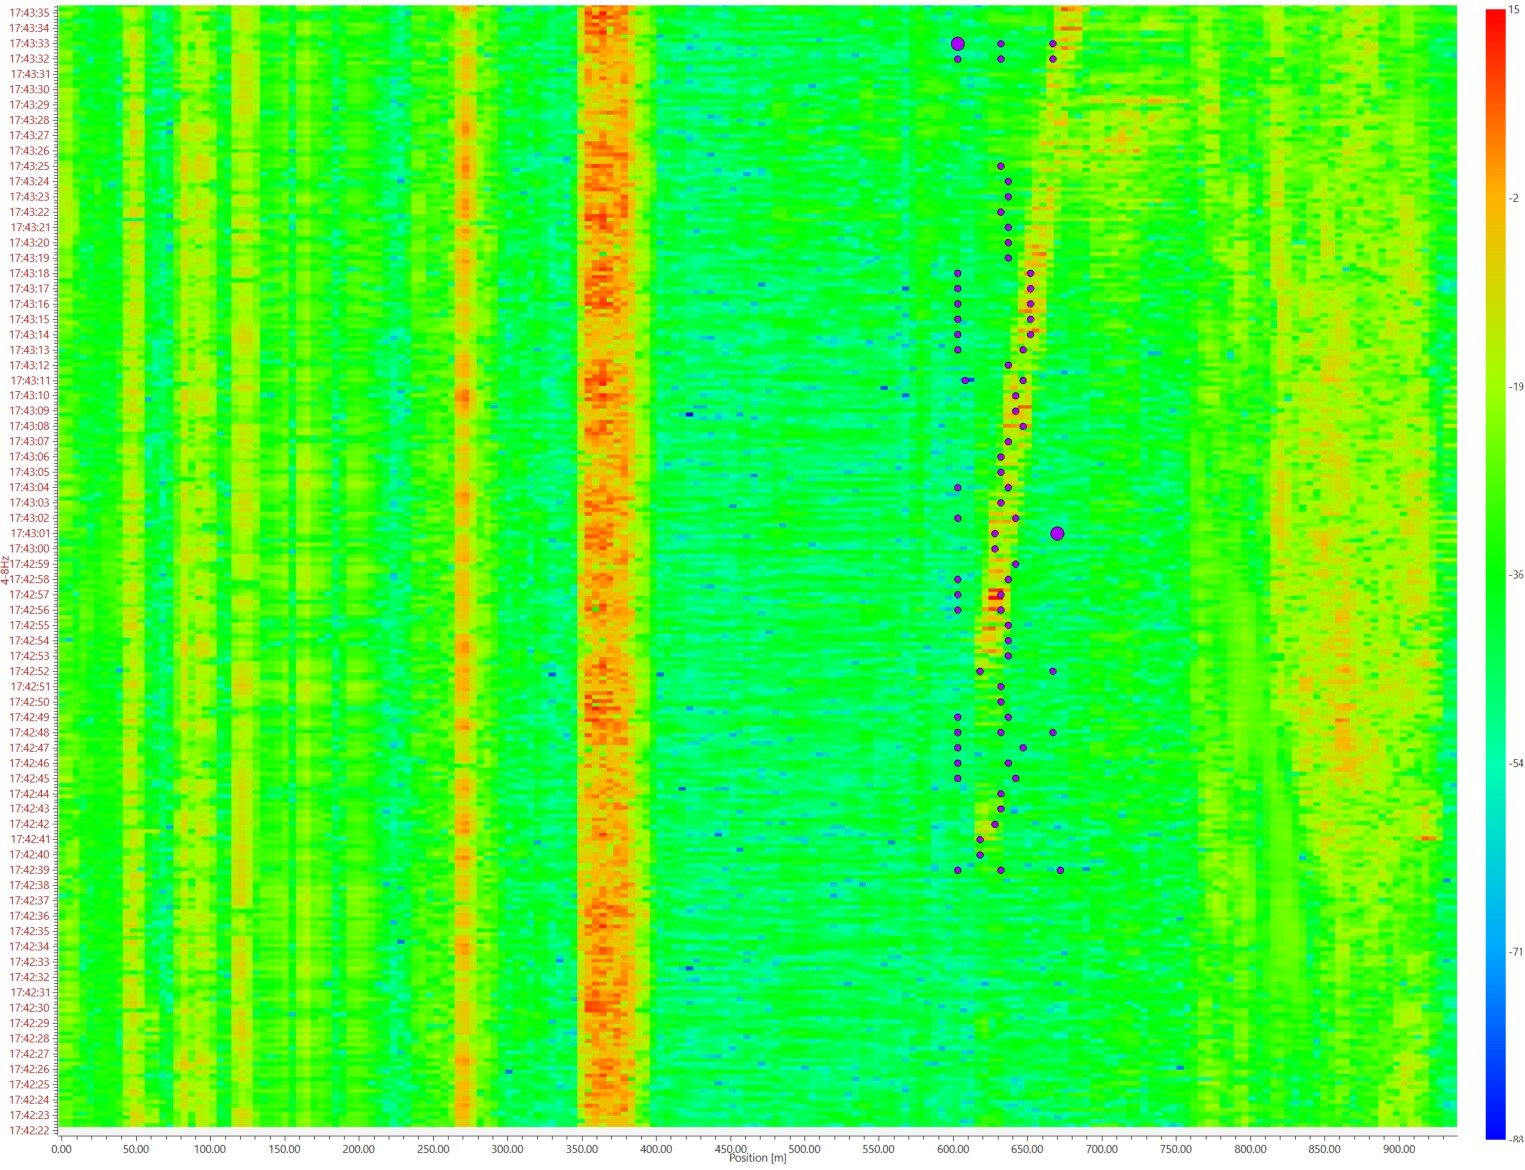
\includegraphics[width=0.9\linewidth]{Bilder/jpg/conv_1d_eval.jpg}
  \caption{DAS Configurator Application detections for ConvNext V2 model on dataset-1D}
  \label{conv_1d_eval}
\end{figure}

The checkpoint file for dataset-1D is loaded into the framework for evaluation. The \texttt{window\_len\_secs} is set to 1.728 seconds and \texttt{hop\_len\_secs} is set to 1 second. Zone is set between 600 to 675 meters to focus on the area as too many detections are generated if the entire files given and application is not able to handle them. Threshold is set to 0.9 to remove the false positives. Figure~\ref{conv_1d_eval} shows the detections after running the evaluation framework on the dataset-1D. 

The detections are shown with the help of purple bubbles. The smaller bubbles are events and bigger bubbles are alarms. As seen in the figure~\ref{conv_1d_eval} there are around 70 detections which shows model is able to detect footsteps but also on the neighboring spatial channels. This shows detections is not perfect as the detections does not align with the footsteps and exact position cannot be determined.

\begin{figure}[h]
  \centering
  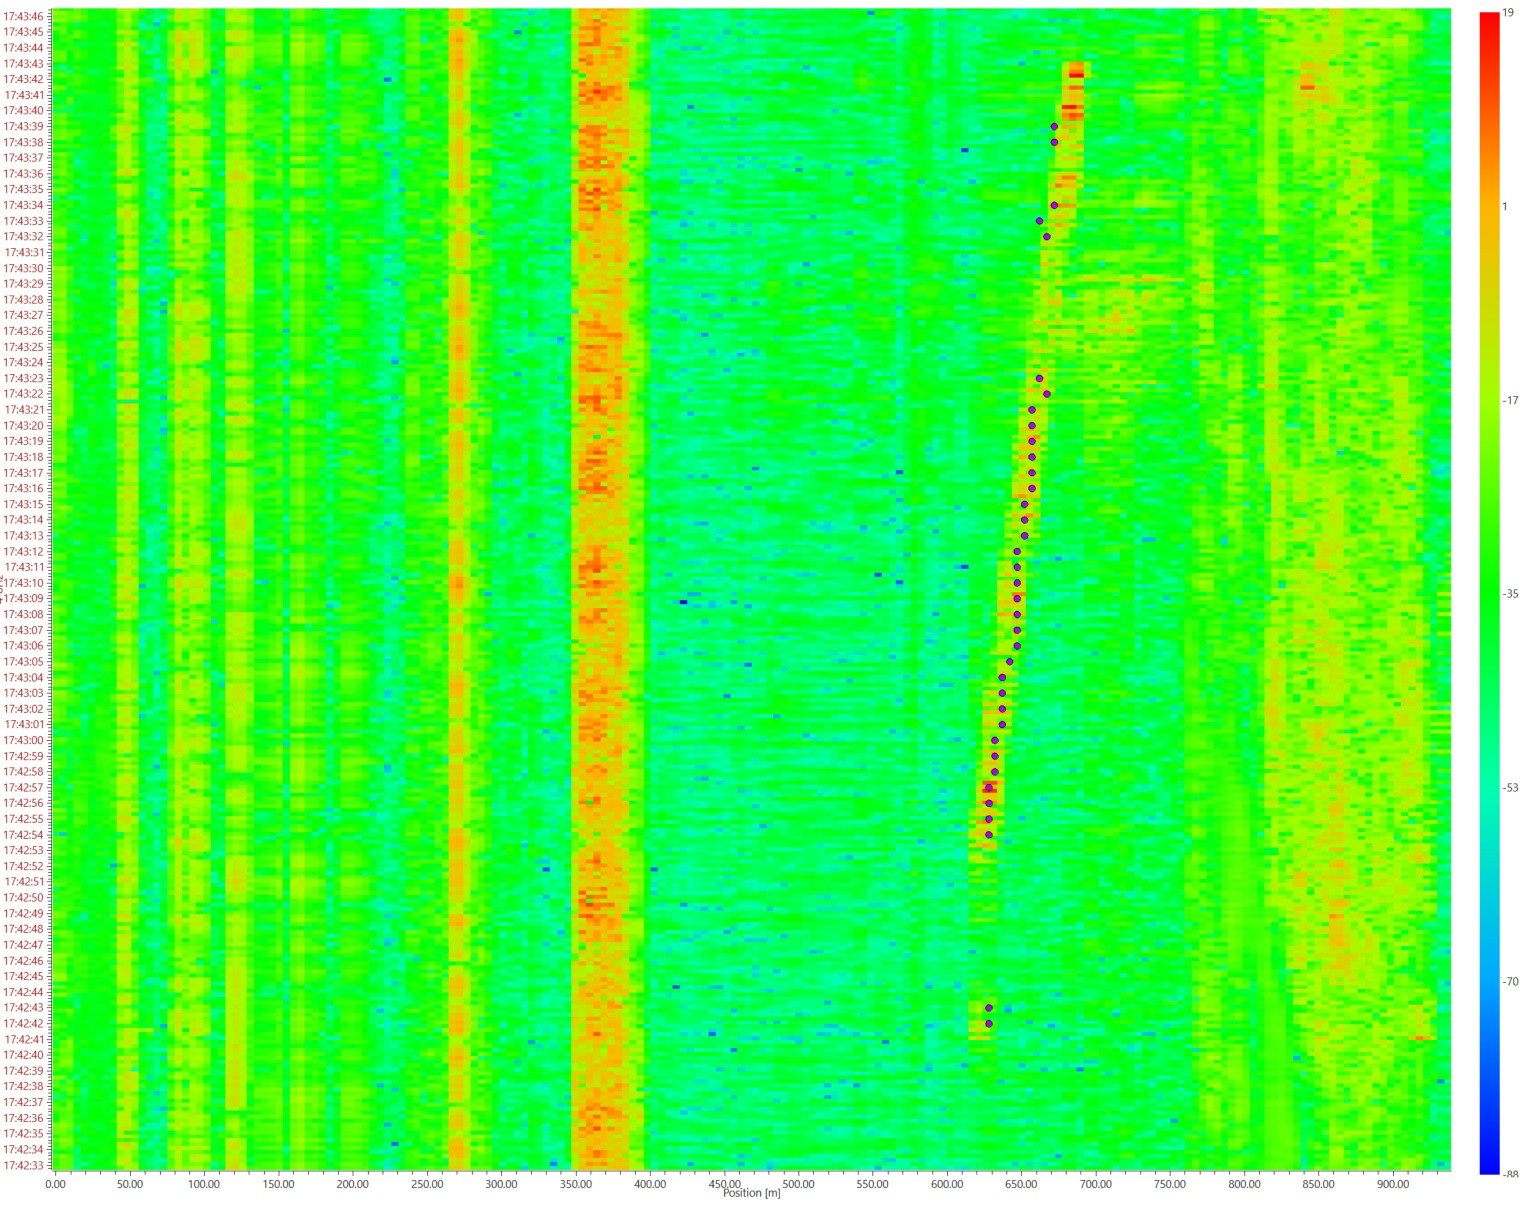
\includegraphics[width=0.9\linewidth]{Bilder/jpg/conv_2d_eval.jpg}
  \caption{DAS Configurator Application detections for ConvNext V2 model on dataset-2D}
  \label{conv_2d_eval}
\end{figure}

Now the checkpoint file for dataset-2D is loaded into the framework for evaluation. The \texttt{window\_len\_secs} and \texttt{hop\_len\_secs} are set to 2 seconds and 1 seconds respectively. Rest of the other parameters are kept the same. Figure~\ref{conv_2d_eval} shows the around 35 detections when evaluation framework is ran. The major difference from dataset-1D is that the footstep trail is more clear and there are lot less false positives with detections more aligned to the actual footstep trail.

From the accuracies over the respective datasets in section~\ref{sec:comp} it was evident that the model with dataset-2D is better than the dataset-1D as the accuracies were 87\% and 99\% respectively. The false positives are much lesser and the footsteps are more accurate in dataset-2D. 

\subsection{EfficientNet Model evaluation}
\label{sec:eff_eval}
EfficientNet Model is also trained in a similar fashion as ConvNext V2 model with dataset-1D and dataset-2D. Models with their respective checkpoints are evaluated by keep The EfficientNet model is selected in the framework in listing~\ref{lst:model_rt} and the number channels are also set according to the checkpoint file. 

\begin{figure}[h]
  \centering
  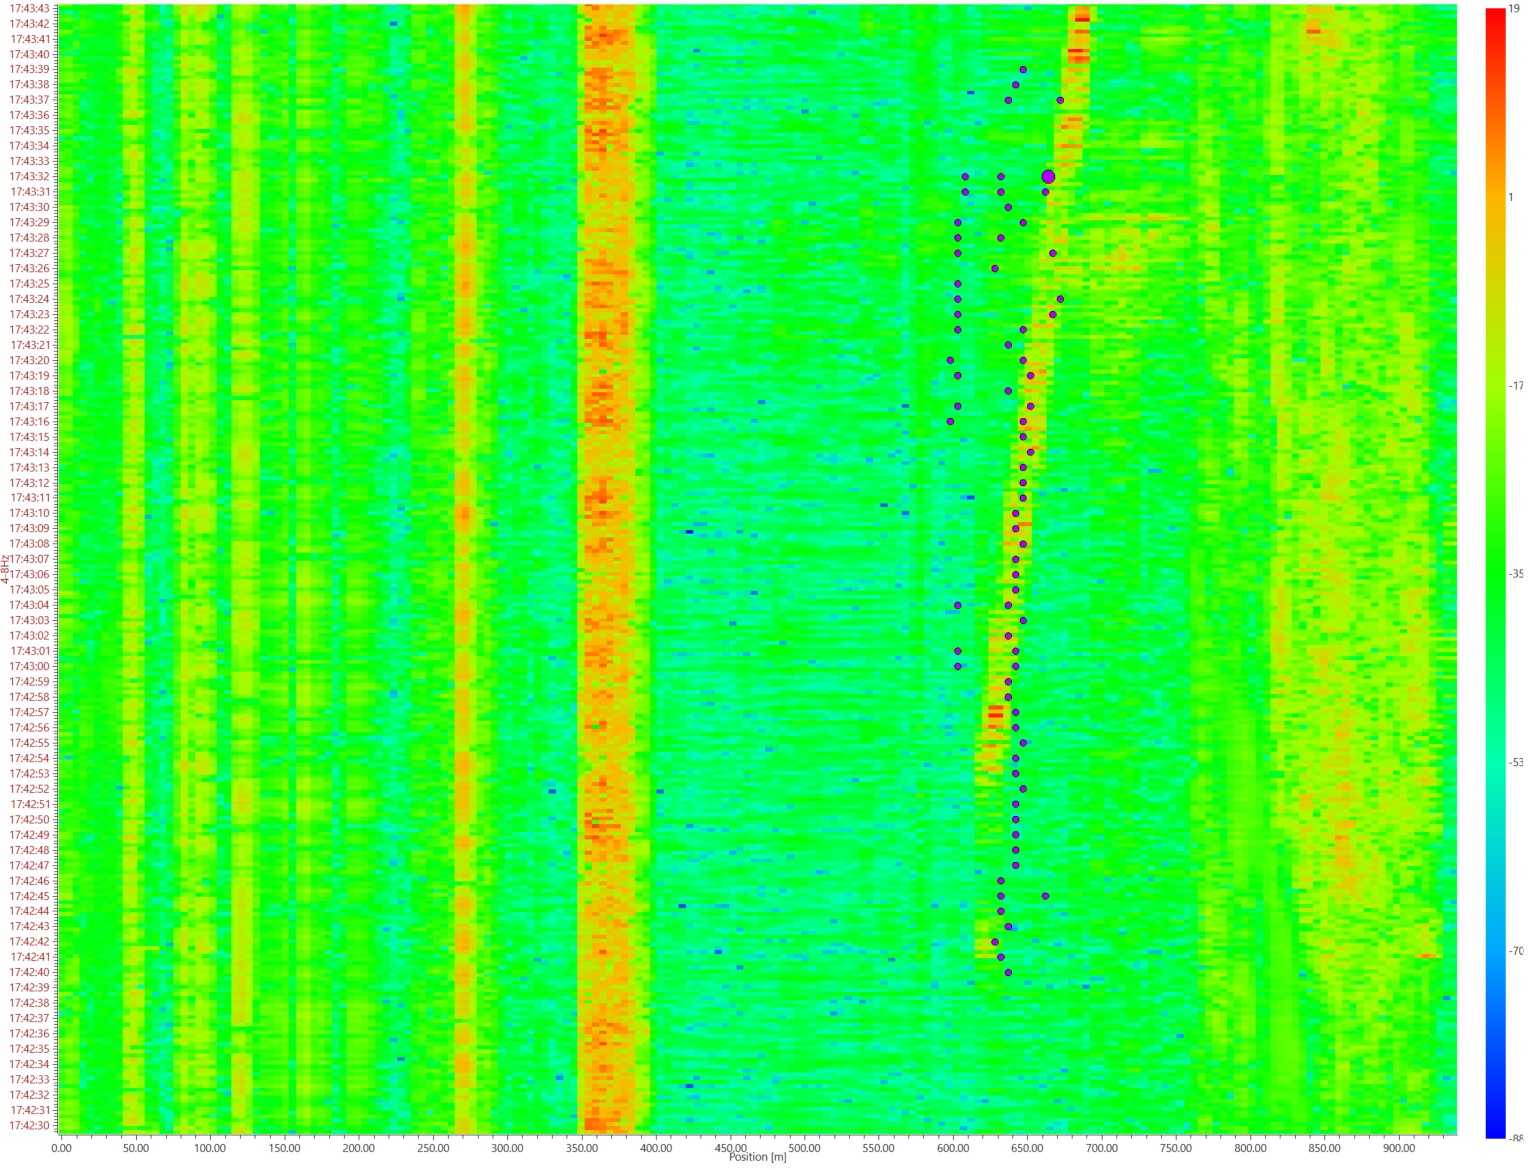
\includegraphics[width=0.9\linewidth]{Bilder/jpg/eff_1d_eval.jpg}
  \caption{DAS Configurator Application detections for EfficientNet V2 model on dataset-1D}
  \label{eff_1d_eval}
\end{figure}

The checkpoint file for dataset-1D is loaded into the framework nad the parameters are setup. The \texttt{window\_len\_secs} is set to 1.728 seconds and \texttt{hop\_len\_secs} is set to 1 second. Zone is selected the same as ConvNext V2 model which is between 600 to 675 meters to focus on a specific region. Threshold value is also kept same to 0.9 to make sure that only the detections with utmost certainty are recorded. 

Figure~\ref{eff_1d_eval} shows the about 70 detections by the model on dataset-1D. Detections are shown with purple bubbles with smaller ones as the events and bigger ones as alarms. The detections are similar to the ConvNext V2 model for dataset-1D. In a similar fashion, the model is able to detect the trail but with it there are lot of false positives on neighboring spatial channel. The exact position of footsteps is not determinable.  

\begin{figure}[h]
  \centering
  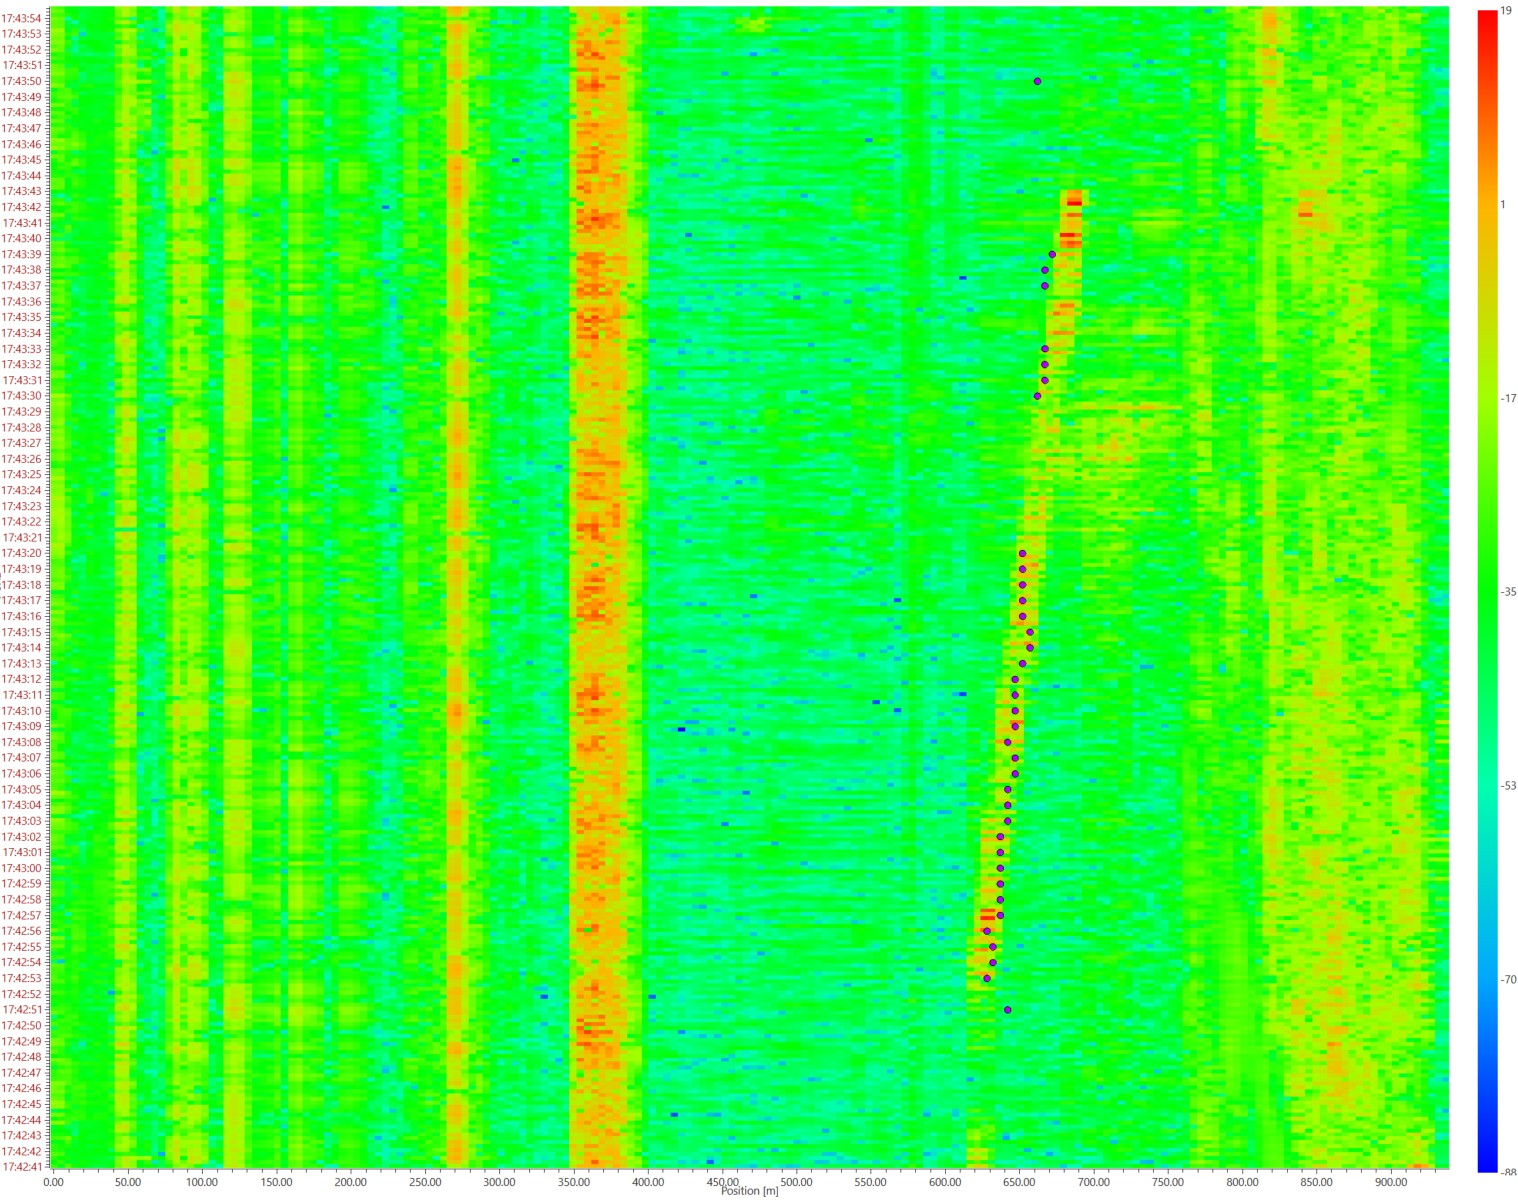
\includegraphics[width=0.9\linewidth]{Bilder/jpg/eff_2d_eval.jpg}
  \caption{DAS Configurator Application detections for EfficientNet V2 model on dataset-2D}
  \label{eff_2d_eval}
\end{figure}

Dataset-2D checkpoint file is loaded into the framework and parameters remain the same. Spatial channels are set to 10. The \texttt{window\_len\_secs} is et to 2 seconds and  \texttt{hop\_len\_secs} is et to 1 seconds. Zone is kept the same to focus on 600 to 675 meters. Threshold is also kept same at 0.9. Figure~\ref{eff_2d_eval} shows about 35 detections made when the evaluation framework is ran. The detections are much more accurate and focused on the footstep trail. Model performs similarly to the ConvNext V2 model on dataset-2D.

The accuracies for the EfficientNet model for dataset-1D and dataset-2D are same (99.43\%). Even though the accuracies are same the detections in dataset-2D model are much more accurate and lesser False positives. 

\section{Comparison of the Model Performances}
The models are evaluated over the framework for both the models and for the checkpoints trained over dataset-1D and dataset-2D in subsections~\ref{sec:conv_eval} and \ref{sec:eff_eval}. The dataset-1D shows about 70 detections and dataset-2D shows about 35 detections. It is evident that the models trained over dataset-2D are performing much better than models trained over dataset-1D with lot less false positives and better localization of footsteps. Even though the accuracies are quite similar for almost every model trained except for the ConvNext v2 model trained over dataset-1D which 87\% this, the dataset-2D models are performing much better. 

The reason for this can be explained the model is trained over dataset-2D has the data with 10 spatial channels because of which the model is able to learn the features of the channel where the detections are made and the model is able to distinguish between the channels. The model focuses on the channel where the footsteps distortions are maximum and not give out the false positives which are observed in the neighboring channels. Same cannot be said for the dataset-1D trained models as the model is trained with only 1 spatial channel. The model doesn't know to distinguish between the channels and gives out the detections when it observes the distortions. The false positives can be much higher if the zone is not fixed and the entire file is given to the model. This can lead to too many detections and application is not able to handle them. Also, if there are too many false positives it becomes difficult to find the actual footstep and thus not able to pin point to the exact location. Each footstep is not detected and model is not trained over very short clips of 3 to 5 footsteps.

Thus from the evaluation results, it is clear that the models trained over 10 spatial channels are preforming better than the models trained over 1 spatial channel irrespective of the model selection.

All results above are evaluated over the 600-675 m zone, where noisy regions are absent. In Figures~\ref{conv_1d_eval}, \ref{conv_2d_eval}, \ref{eff_1d_eval}, and \ref{eff_2d_eval}, the 350-400 m segment (highlighted in red) exhibits elevated background noise, leading to random false positive detections. Raising the confidence threshold (\texttt{min\_prob}) reduces these spurious alarms but risks missing faint footsteps, especially outside the clean zone.

